\documentclass[../AnalisideiRequisiti.tex]{subfiles}

\begin{document}
	% Il comando UserCase accetta primo una label nel caso serva un link verso di lui \refer{label} poi 
	% attore primario
	% attore secondario
	% Descrizione
	% Precondi
	% Post
	% Scenario principale
	% Scenari alternativi 

	\chapter{Casi d'uso}
	\section{Classificazione dei casi d'uso}
	I casi d'uso sono identificati da un codice descritto nelle NP (§2.2.3.4).
	Di seguito viene visualizzato il diagramma generale dei casi d'uso del sistema. 
	
	\section{Visione generale del sistema}
	Segue un diagramma dei casi d'uso che riassume la visione generale del sistema da sviluppare. Le sezioni successive esaminano invece i singoli casi d'uso individuati.
	
	\begin{figure}[H]
	\centering	
	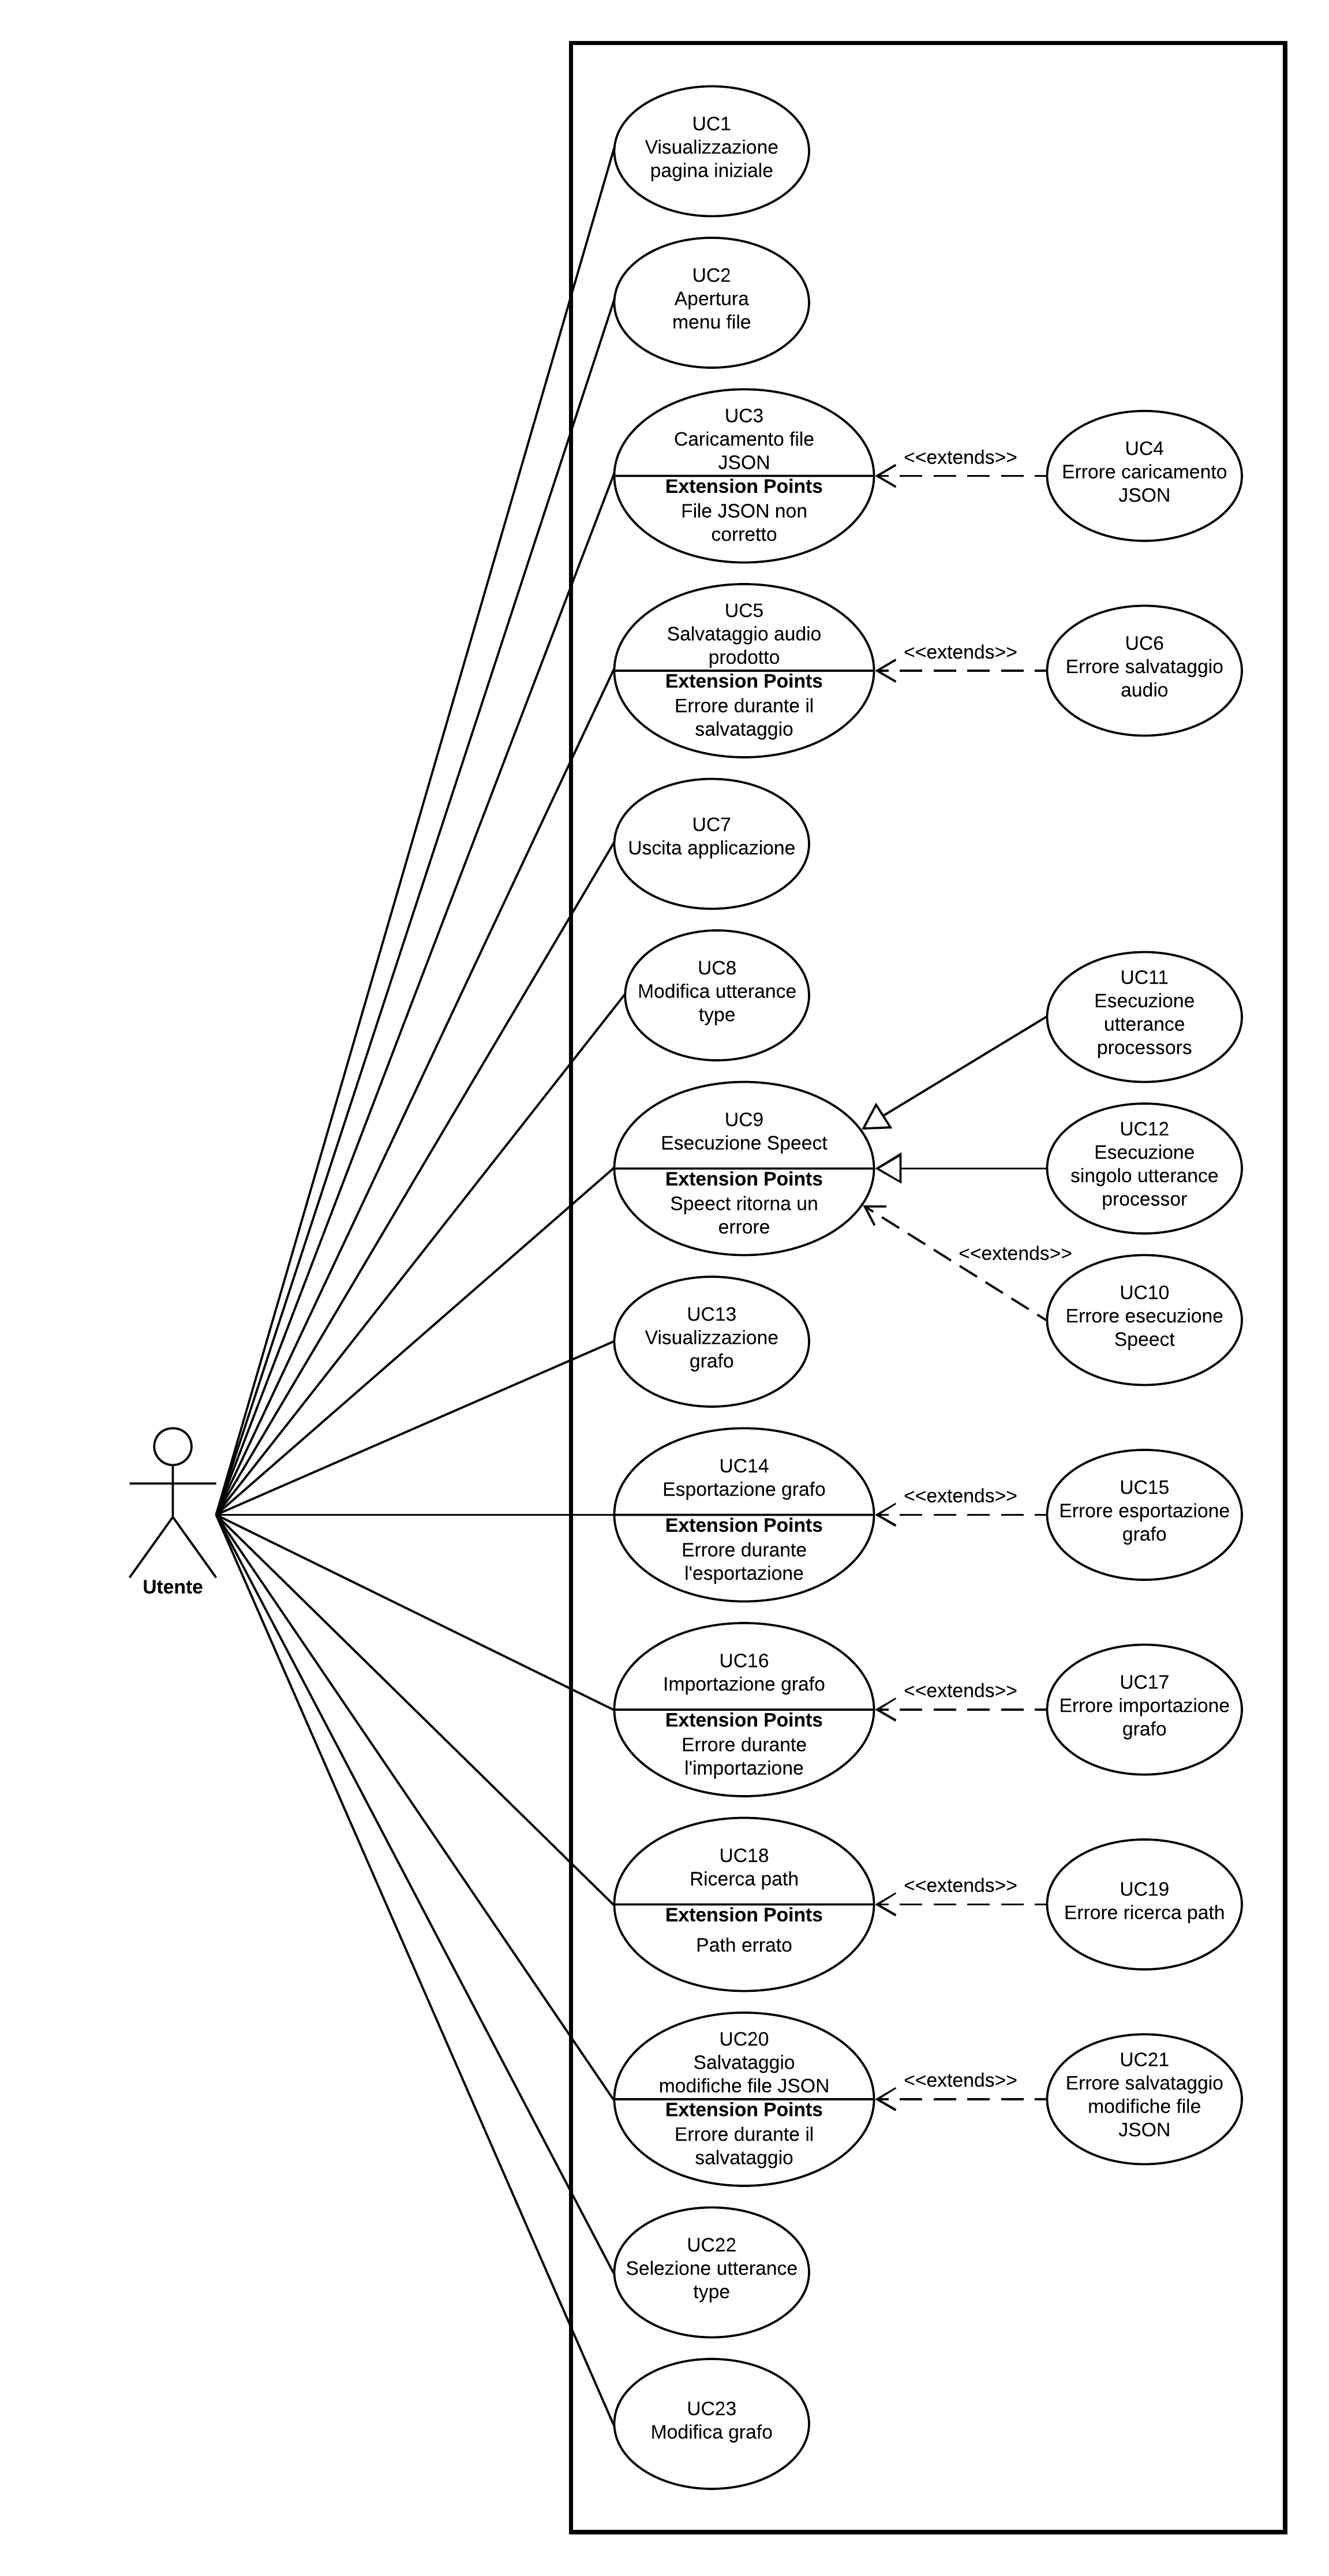
\includegraphics[scale=0.52]{../img/UC.png}
	
	\caption{Visione generale del sistema}
	
	\end{figure}
 	
	\section{UC1: Visualizzazione pagina iniziale} 
		
	\UserCase
	{UC1}
	{Utente}
	{Non previsto}
	{L'attore visualizza la pagina iniziale di DeSpeect dalla quale può aprire il menu File, caricare un file \verb|.json|, selezionare l'utterance type, scrivere del testo in input, eseguire Speect, modificare l'utterance type e modificare il grafo}
	{DeSpeect è stato avviato}
	{Viene visualizzata la pagina iniziale di DeSpeect}
	{\begin{itemize}
			\item{} L'attore può aprire il menù File \refer{UC2};
			\item{} L'attore può caricare un file \verb|.json| \refer{UC3};
			\item{} L'attore può selezionare l'utterance type \refer{UC22};
			\item{} L'attore può modificare l'utterance type \refer{UC8};
			\item{} L'attore può scrivere del testo in input;
			\item{} L'attore può eseguire Speect \refer{UC9};
			\item{} L'attore può modificare il grafo \refer{UC23}.
	\end{itemize}}
	{Non previsti}
	
	
	\section{UC2: Apertura menù File}

	\UserCase
	{UC2}
	{Utente}
	{Non previsto}
	{L'attore visualizza il menù File, dal quale può caricare o salvare un file \verb|.json|, caricare o salvare un grafo, salvare l'audio prodotto, cercare il percorso di un nodo nel grafo e chiudere l'applicazione}
	{L'attore clicca sul menù File}
	{Il menù File è aperto e visualizza le voci corrispondenti}
	{	\begin{itemize}
		\item{} L'attore può caricare un file \verb|.json| \refer{UC3};
		\item{} L'attore può salvare le modifiche al file \verb|.json| \refer{UC20};
		\item{} L'attore può caricare un grafo \refer{UC16};
		\item{} L'attore può salvare un grafo \refer{UC14};
		\item{} L'attore può salvare l'audio prodotto da Speect \refer{UC5};
		\item{} L'attore può cercare il percorso di un nodo nel grafo \refer{UC18};
		\item{} L'attore può chiudere l'applicazione \refer{UC7}.
		\end{itemize}
	}
	{Non previsti}

	\section{UC3: Caricamento file .json}
	\UserCase
	{UC3}
	{Utente}
	{Non previsto}
	{L'attore vuole caricare un file \verb|.json|}
	{L'attore ha selezionato la voce relativa nel menù \refer{UC2}}
	{Viene inizializzato Speect con il file \verb|.json| selezionato e aggiornata la GUI}
	{
		\begin{itemize}
			\item{} Viene aperto il file browser;
			\item{} L'attore seleziona il file;
			\item{} L'attore conferma la selezione;
			\item{} Il file viene dato a Speect che tenta l'inizializzazione;
			\item{} Viene visualizzato il percorso del file nell'apposito spazio \ref{fig:GUI}.
		\end{itemize}
	}
	{Speect fallisce l'inizializzazione e l'attore visualizza il messaggio d'errore relativo al file \refer{UC4}}
	
	\section{UC4: Errore caricamento file .json}
	\UserCase
	{UC4}
	{Utente}
	{Non previsto}
	{Durante l'inizializzazione, Speect fallisce ritornando un errore}
	{L'attore carica un file \verb|.json| non corretto}
	{L'errore è visualizzato a schermo e viene ripristinato lo stato precedente, ridando controllo all'attore}
	{L'attore ha caricato un file \verb|.json| non corretto e viene visualizzato un messaggio di errore}
	{Non previsti}

\section{UC5: Salvataggio audio prodotto}
\UserCase
{UC5}
{Utente}
{Non previsto}
{L'attore vuole salvare l'audio prodotto}
{Speect è inizializzato \refer{UC3}}
{L'audio è salvato in un file}
{
		\begin{itemize}
		\item{} Viene aperto il file browser;
		\item{} L'attore si sposta nella cartella di destinazione;
		\item{} L'attore scrive il nome del file nella barra di testo dedicata;
		\item{} L'attore conferma il salvataggio;
		\item{} Speect compila producendo il file desiderato;
		\item{} Il file viene salvato nella destinazione con estensione \verb|.wav|.
		\end{itemize}
}
{Avviene un errore durante il salvataggio dell'audio e l'attore visualizza il messaggio di errore relativo \refer{UC6}}
		
\section{UC6: Errore salvataggio audio}
\UserCase
{UC6}
{Utente}
{Non previsto}
{Avviene un errore durante il salvataggio dell'audio}
{L'attore ha cercato di salvare il file audio prodotto} 
{Viene visualizzato l'errore e nessuna operazione viene eseguita}
{L'attore ha cercato di salvare il file audio prodotto e viene visualizzato un messaggio di errore}
{Non previsti}

\section{UC7: Uscita applicazione}
\UserCase
{UC7}
{Utente}
{Non previsto}
{L'attore, che vuole chiudere l'applicazione, visualizza una finestra di conferma e convalida la chiusura dell'applicazione}
{L'applicazione è in esecuzione}
{L'attore conferma la chiusura dell'applicazione e l'applicazione viene terminata}
{Chiusura dell'applicazione}
{L'attore annulla la chiusura dell'applicazione}

\section{UC8: Modifica utterance type}
\begin{figure}[H]
	\centering
	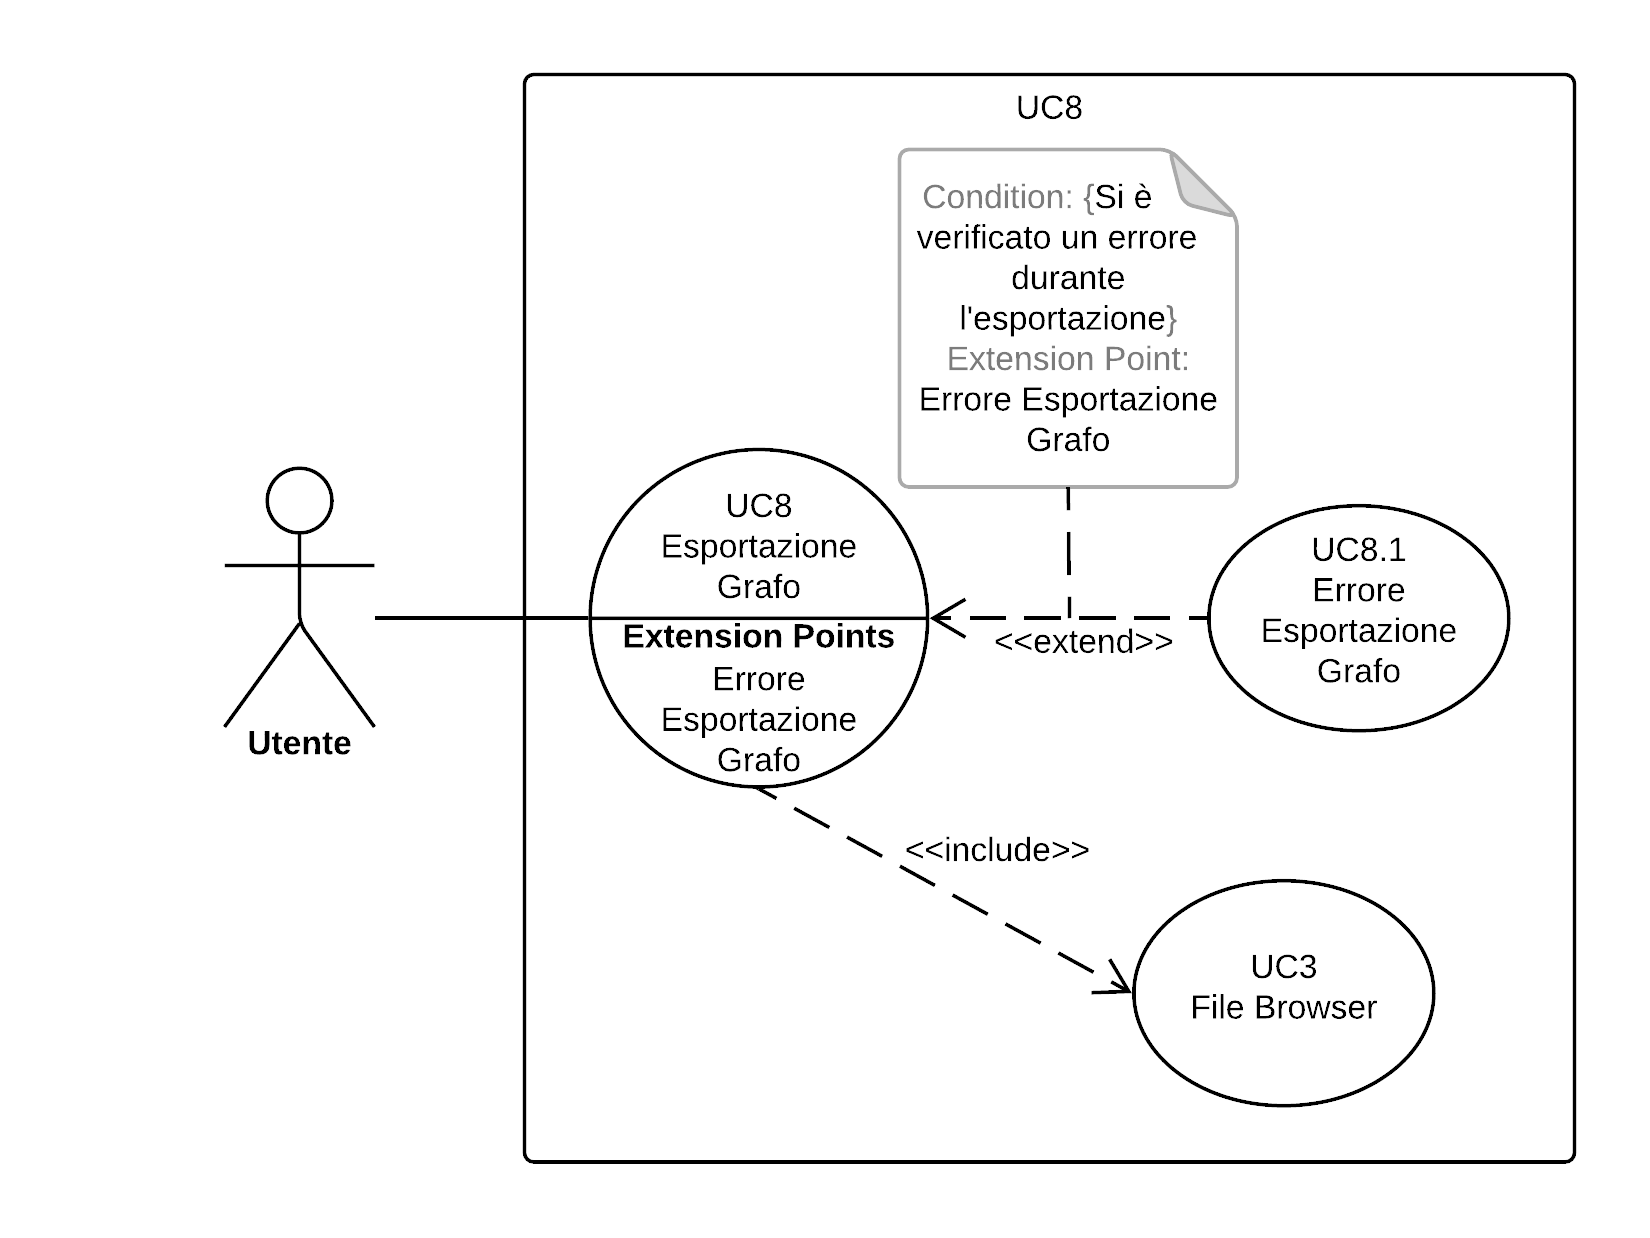
\includegraphics[width=\textwidth]{../img/UC8.png}
	\caption{UC8: Modifica utterance type}
\end{figure}
\UserCase
{UC8}
{Utente}
{Non previsto}
{L'attore vuole modificare l'utterance type}
{\'E presente almeno un'utterance type e questa è selezionata \refer{UC22}}
{L'utterance type è stata modificata e il file \verb|.json| viene aggiornato}
{
	\begin{itemize}
		\item{} L'attore seleziona un utterance processor;
		\item{} L'attore riordina o rimuove l'utterance processor;	
		\item{} Le operazioni vengono eseguite;
		\item{} Il file \verb|.json| relativo viene aggiornato.	
	\end{itemize}
}
{Non previsti}

\section{UC8.1: Selezione utterance processor}
\UserCase
{UC8.1}
{Utente}
{Non previsto}
{L'attore vuole selezionare un utterance processor per spostarlo}
{Un file \verb|.json| è stato caricato correttamente \refer{UC3}}
{Vengono visualizzati i bottoni per modificare tale utterance processor}
{
	\begin{itemize}
		\item{} L'attore clicca sul nome dell'utterance processor;
		\item{} Vengono visualizzati due bottoni che permettono lo spostamento grafico del utterance processor \refer{UC8.2} e un bottone che ne permette la rimozione \refer{UC8.3}. 		
	\end{itemize}
}
{Non previsti}

\section{UC8.2: Riordino utterance processor}
\UserCase
{UC8.2}
{Utente}
{Non previsto}
{L'attore vuole cambiare l'ordine degli utterance processor}
{L'attore ha selezionato un utterance processor \refer{UC8.1}}
{Il file \verb|.json| viene aggiornato}
{
	\begin{itemize}
		\item{} L'attore clicca sull'utterance processor \refer{UC8.1};
		\item{} L'attore lo riordina tramite i pulsanti forniti;
		\item{} Le operazioni vengono eseguite;
		\item{} Se esisteva un grafo, esso non viene modificato.
		
	\end{itemize}
}
{Non previsti}

\section{UC8.3: Rimozione utterance processor}
\UserCase
{UC8.3}
{Utente}
{Non previsto}
{L'attore vuole rimuovere un utterance processor}
{L'attore ha selezionato un utterance processor \refer{UC8.1}}
{Il file \verb|.json| viene aggiornato}
{
	\begin{itemize}
		\item{} L'attore clicca sull'utterance processor \refer{UC8.1};
		\item{} L'attore lo rimuove tramite il pulsante fornito;
		\item{} L'operazione viene eseguita;
		\item{} Se esisteva un grafo, esso non viene modificato.
		
	\end{itemize}
}
{Non previsti}

\section{UC9: Esecuzione Speect}
\UserCase
{UC9}
{Utente}
{Non previsto}
{L'attore vuole eseguire Speect}
{Il file \verb|.json| è stato caricato correttamente \refer{UC3}}
{Speect elabora il testo selezionato e viene visualizzato il grafo}
{\begin{itemize}
		\item{} L'attore seleziona l'utterance type \refer{UC22};
		\item{} L'attore compila il campo di testo o inserisce un grafo HRG;
		\item{} L'attore preme sul tasto di esecuzione;
		\item{} Vengono eseguiti gli utterance processor selezionati;
		\item{} Viene mostrato il grafo risultante dall'esecuzione \refer{UC13}.
	\end{itemize}
}
{Speect ha fallito l'esecuzione e l'attore visualizza un messaggio di errore \refer{UC10}}

\section{UC10: Errore esecuzione Speect}
\UserCase
{UC10}
{Utente}
{Non previsto}
{L'attore visualizza a schermo l'errore di esecuzione di Speect}
{Speect ha fallito l'esecuzione}
{Viene visualizzato un messaggio di errore}
{L'attore ha provato ad eseguire Speect e viene visualizzato un messaggio di errore}
{Non previsti}

\section{UC11: Esecuzione utterance processors}
\UserCase
{UC11}
{Utente}
{Non previsto}
{Speect esegue gli utterance processors selezionati}
{Un'utterance type è stata selezionata \refer{UC22} }
{Vengono eseguiti gli utterance processors partendo dal grafo già presente o dal campo di testo scritto}
{
	\begin{itemize}
		\item{} L'attore seleziona gli utterance processors \refer{UC8.1};
		\item{} L'attore può compilare il campo di testo;
		\item{} L'attore preme sul tasto di esecuzione.
	\end{itemize}
}
{Speect ha fallito l'esecuzione}

\section{UC12: Esecuzione singolo utterance processor}
\UserCase
{UC12}
{Utente}
{Non previsto}
{Speect esegue un singolo utterance processor}
{Un'utterance type è stata selezionata \refer{UC22} }
{Viene eseguito l'utterance processor partendo dal grafo già presente o dal campo di testo scritto}
{
	\begin{itemize}
		\item{} L'attore seleziona l'utterance processor \refer{UC8.1};
		\item{} L'attore può compilare il campo di testo;
		\item{} L'attore preme sul tasto di esecuzione per il singolo processor \ref{fig:GUI}.
	\end{itemize}
}
{Speect ha fallito l'esecuzione}

\section{UC13: Visualizzazione grafo}
\UserCase
{UC13}
{Utente}
{Non previsto}
{L'attore visualizza il grafo}
{Speect ha terminato l'esecuzione con successo \refer{UC9}}
{Viene visualizzato a schermo un grafo corretto con almeno un nodo cliccabile}
{
	L'attore visualizza il grafo corretto e può modificarlo \refer{UC23}
}
{Non previsti}


\section{UC14: Esportazione grafo}
\UserCase
{UC14}
{Utente}
{Non previsto}
{L'attore vuole esportare il grafo visualizzato}
{Esiste un grafo esportabile}
{Il grafo viene esportato in un file}
{
	\begin{itemize}
			\item{} Viene aperto il file browser;
			\item{} L'attore si sposta nella cartella in cui salvare il grafo;
			\item{} L'attore scrive il nome del file nella barra di testo dedicata;
			\item{} L'attore conferma il salvataggio.
	\end{itemize}
}
{L'esportazione fallisce e l'attore visualizza un messaggio di errore \refer{UC15}}

\section{UC15: Errore esportazione grafo}
\UserCase
{UC15}
{Utente}
{Non previsto}
{Avviene un errore durante l'esportazione}
{L'esportazione del grafo è fallita}
{Viene visualizzato un messaggio di errore e nessuna operazione viene eseguita}
{L'esportazione del grafo è fallita e viene visualizzato un messaggio di errore}
{Non previsti}

\section{UC16: Importazione grafo}

\UserCase
{UC16}
{Utente}
{Non previsto}
{L'attore vuole importare un grafo}
{Esiste un grafo e l'attore ha cliccato su Carica Grafo \refer{UC2}}
{Il grafo viene importato da file}
{
	\begin{itemize}
			\item{} Viene aperto il file browser;
			\item{} L'attore seleziona il file da importare;
			\item{} L'attore conferma l'apertura del file.
	\end{itemize}
}
{L'importazione fallisce e l'attore visualizza un messaggio di errore \refer{UC17}}

\section{UC17: Errore importazione grafo}
\UserCase
{UC17}
{Utente}
{Non previsto}
{Avviene un errore durante l'importazione}
{L'importazione del grafo è fallita}
{Viene visualizzato l'errore e nessuna operazione viene eseguita}
{L'importazione del grafo è fallita e viene visualizzato un messaggio di errore}
{Non previsti}

\section{UC18: Ricerca path}

\UserCase
{UC18}
{Utente}
{Non previsto}
{L'attore vuole cercare un nodo tramite un percorso nel grafo}
{Esiste un grafo corretto, l'attore ha selezionato un nodo e premuto Ricerca Path nel menu File}
{Se il path porta ad un nodo definito, esso viene evidenziato}
{
	\begin{itemize}
		\item{} Viene visualizzata una finestra con una casella di testo e un pulsante;
		\item{} L'attore inserisce il percorso da cercare;
		\item{} L'attore preme il pulsante di Ricerca;
		\item{} Se il percorso inizia dal nodo selezionato e finisce in un nodo esistente, il nodo di arrivo viene evidenziato.
 	\end{itemize}
}
{Il percorso inserito dall'attore non è corretto e viene visualizzato un errore \refer{UC19}}

\section{UC19: Errore ricerca path}
\UserCase
{UC19}
{Utente}
{Non previsto}
{L'attore vuole cercare un nodo tramite un percorso nel grafo}
{Il percorso inserito dall'attore è sintatticamente errato}
{Viene visualizzato l'errore a schermo e si riapre la finestra di Ricerca \refer{UC18}}
{Il percorso inserito dall'attore non è corretto e viene visualizzato un messaggio di errore}
{Non previsti}

\section{UC20: Salvataggio modifiche file .json}

\UserCase
{UC20}
{Utente}
{Non previsto}
{L'attore ha modificato gli utterance processor e vuole salvare il nuovo file \verb|.json|}
{Esiste un file \verb|.json| correttamente caricato \refer{UC3} e l'attore ha modificato gli utterance processor \refer{UC8.2} \refer{UC8.3}}
{Le modifiche vengono salvate}
{
	\begin{itemize}
		\item{} L'attore apre il menu File \refer{UC2};
		\item{} L'attore preme su Salva File JSon.
	\end{itemize}
}
{L'operazione di salvataggio fallisce e viene visualizzato un errore \refer{UC21}}

\section{UC21: Errore salvataggio modifiche file .json}
\UserCase
{UC21}
{Utente}
{Non previsto}
{L'attore ha provato a salvare il file \verb|.json|}
{L'operazione di salvataggio fallisce}
{Viene visualizzato l'errore e nessuna operazione viene eseguita}
{L'operazione di salvataggio fallisce e viene visualizzato un errore}
{Non previsti}

\section{UC22: Selezione utterance type}
\UserCase
{UC22}
{Utente}
{Non previsto}
{L'attore vuole selezionare l'utterance type desiderata}
{Un file \verb|.json| è stato caricato correttamente \refer{UC3}}
{Vengono mostrati gli utterance processors utilizzati da Speect per tale utterance type}
{
	\begin{itemize}
		\item{} L'attore apre il menu a tendina relativo;
		\item{} L'attore clicca sull'utterance type desiderata;
		\item{} Vengono mostrati a schermo i nomi degli utterance processor utilizzati, negli appositi spazi \ref{fig:GUI}.
	\end{itemize}
}
{Non previsti}

\section{UC23: Modifica grafo}
\begin{figure}[H]
	\centering
	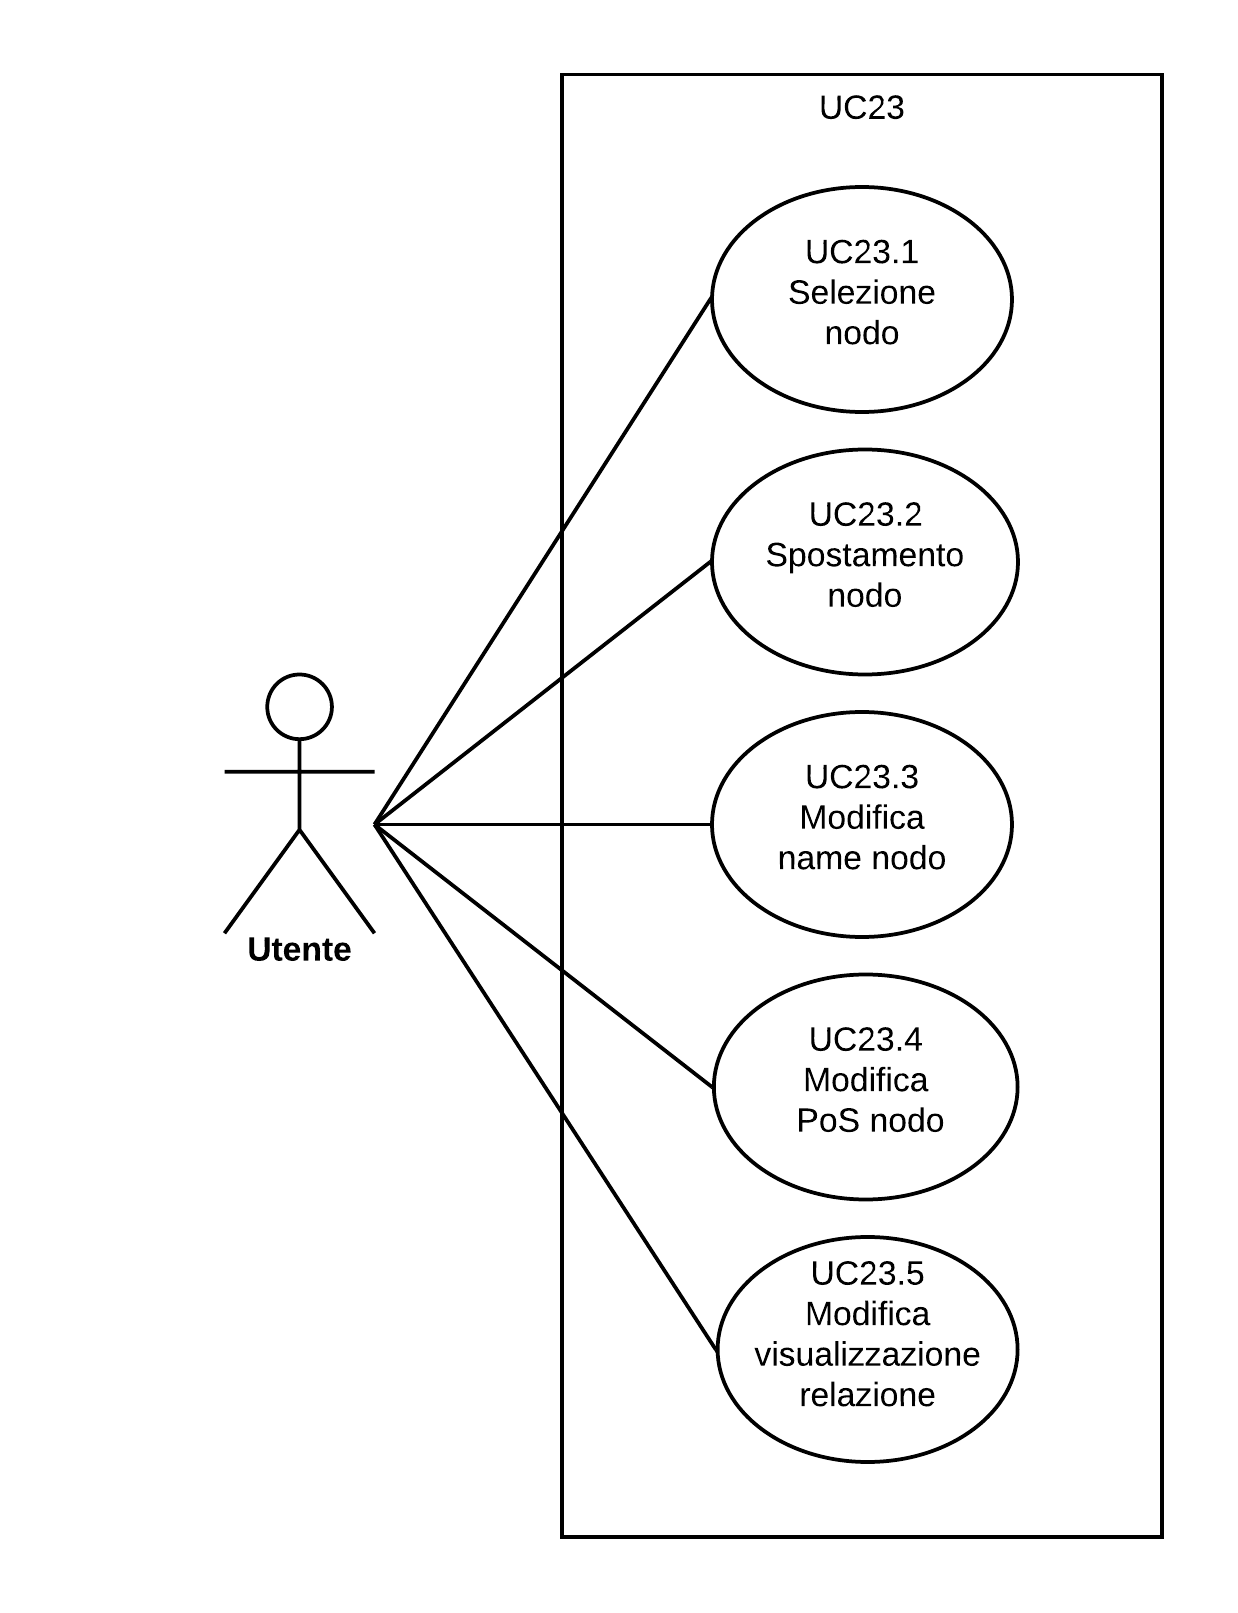
\includegraphics[width=\textwidth]{../img/UC23.png}
	\caption{UC23: Modifica grafo}
\end{figure}
\UserCase
{UC23}
{Utente}
{Non previsto}
{L'attore vuole modificare il grafo}
{Viene visualizzato a schermo un grafo corretto con almeno un nodo cliccabile \refer{UC13}}
{Il grafo è stato modificato}
{
	L'attore per modificare un grafo può:
	\begin{itemize}
		\item{} selezionare un nodo \refer{UC23.1};
		\item{} spostare un nodo \refer{UC23.2};	
		\item{} modificare un nodo \refer{UC23.3} \refer{UC23.4};	
		\item{} modificare la visualizzazione delle relazioni \refer{UC23.5}.		
	\end{itemize}
}
{Non previsti}

\section{UC23.1: Selezione nodo}
\UserCase
{UC23.1}
{Utente}
{Non previsto}
{L'attore vuole selezionare un nodo per visualizzarne i dettagli}
{Viene visualizzato a schermo un grafo corretto con almeno un nodo cliccabile \refer{UC13}}
{Viene evidenziato il nodo del grafo e vengono mostrate le sue informazioni nella parte della GUI dedicata (\ref{fig:GUI})}
{
	\begin{itemize}
		\item{} L'attore clicca una volta sul nodo;
		\item{} Il nodo viene evidenziato;
		\item{} Nel riquadro apposito (\ref{fig:GUI}) vengono visualizzati i dati del grafo:
		\begin{enumerate}
			\item{} Name;
			\item{} Part of Speech;
		\end{enumerate}
		\item{} L'attore può modificare il name del nodo selezionato \refer{UC23.3};
		\item{} L'attore può modificare il PoS del nodo selezionato \refer{UC23.4}.
	\end{itemize}
}
{Non previsti}

\section{UC23.2: Spostamento nodo}
\UserCase
{UC23.2}
{Utente}
{Non previsto}
{L'attore vuole spostare graficamente un nodo}
{Un nodo è selezionato \refer{UC23.1}}
{Il nodo viene spostato}
{
	\begin{itemize}
		\item{} L'attore trascina il nodo cliccando senza rilasciare;
		\item{} Il nodo si sposta;
		\item{} L'attore rilascia il click;
		\item{} Il nodo rimane nella nuova posizione.
	\end{itemize}
}
{Non previsti}

\section{UC23.3: Modifica name nodo}
\UserCase
{UC23.3}
{Utente}
{Non previsto}
{L'attore vuole modificare il name del nodo selezionato}
{Un nodo è selezionato \refer{UC23.1}}
{Il nodo cambia name}
{
	\begin{itemize}
		\item{} L'attore seleziona la casella di testo del name;
		\item{} L'attore cancella il name precedente;
		\item{} L'attore inserisce il nuovo name;
		\item{} L'attore rimuove il focus dalla casella di testo;
		\item{} Il name viene aggiornato;
		\item{} Il grafo viene aggiornato e ristampato a schermo \refer{UC13}.
	\end{itemize}
}
{Non previsti}

\section{UC23.4: Modifica PoS nodo}
\UserCase
{UC23.4}
{Utente}
{Non previsto}
{L'attore vuole modificare il PoS del nodo selezionato}
{Un nodo è selezionato \refer{UC23.1}}
{Il nodo cambia PoS}
{
	\begin{itemize}
		\item{} L'attore seleziona la casella di testo del PoS;
		\item{} L'attore cancella il PoS precedente;
		\item{} L'attore inserisce il nuovo PoS
		\item{} L'attore rimuove il focus dalla casella di testo;
		\item{} Il PoS viene aggiornato;
		\item{} Il grafo viene aggiornato e ristampato a schermo \refer{UC13}.
	\end{itemize}
}
{Non previsti}

\section{UC23.5: Modifica visualizzazione relazione}
\UserCase
{UC23.5}
{Utente}
{Non previsto}
{L'attore vuole filtrare le relazioni del grafo}
{Un'utterance type è stata scelta \refer{UC22}}
{Vengono mostrati nel grafo tutti i layer di relazione selezionati}
{
	\begin{itemize}
		\item{} L'attore seleziona/deseleziona una checkbox adiacente ad una relazione;
		\item{} La relazione in questione viene visualizzata/nascosta;
		\item{} Il grafo viene aggiornato e ristampato a schermo \refer{UC13}.
	\end{itemize}
}
{Non previsti}

\end{document}
